\documentclass{ximera}
\usepackage{OERLinearAlgebra}


\usepackage{mathtools}
\usepackage{tikz-3dplot}
\newcommand\norm[1]{\left\lVert#1\right\rVert}

\author{Anna Davis \and Rosemarie Emanuele} \title{Introduction to Vectors} \license{CC-BY 4.0}

\begin{document}

\begin{abstract}
 We introduce vectors, and notation associated with vectors in standard position.
\end{abstract}
\maketitle




\section*{What is a Vector?}

A \dfn{scalar} is a quantity that has size, often called  magnitude, but no direction.  For example, temperature, mass and speed are scalars.  A \dfn{vector} has magnitude and direction.  For example, velocity is a vector because it tells us how fast the object is traveling and also the direction of travel.  

If an object is traveling along a number line, the direction of travel is given by the sign of its velocity (positive or negative), while the speed is given by the absolute value of the velocity.  If the object is traveling in a plane or in space, direction of travel can be described by an arrow, while the speed can be represented by the length of the arrow.  Graphically speaking, vectors in $\RR^2$ and $\RR^3$ look like this: 

\begin{image}[4in]
\begin{tikzpicture}[scale=0.8]

  \draw[<->] (-4,0)--(4,0);
  \draw[<->] (0,-4)--(0,4);
  
\draw[line width=2pt,blue,-stealth](1,2)--(-1,3);
 %\draw[line width=2pt,blue,-stealth](-2,-3)--(2,1);
\end{tikzpicture}
\tdplotsetmaincoords{70}{130}
\begin{tikzpicture}
	\draw[->](-2,0,0)--(5,0,0) node[below left]{$y$};
    \draw[->](0,-2,0)--(0,5,0) node[below left]{$z$};
    \draw[->](0,0,-2)--(0,0,5) node[below left]{$x$};
        %\draw[->, line width=2pt,blue, -stealth](-2,3,-2)--(4,3,4);
    \draw[->, line width=2pt,blue, -stealth](2,1,3)--(3,2,-2);
    \draw[dashed](2,1,3)--(2,0,3);
    \draw[dashed](2,0,0)--(2,0,3);
    \draw[dashed](0,0,3)--(2,0,3);
    \draw[dashed](3,2,-2)--(3,0,-2);
    \draw[dashed](3,0,0)--(3,0,-2);
    \draw[dashed](0,0,-2)--(3,0,-2);
    \end{tikzpicture}
\end{image}

A vector can be denoted by a lower-case letter with an arrow over the top (like this: $\overrightarrow{u}$ ), or a bold lower-case letter (like this: $\vec{u}$).  

The magnitude, or length, of a vector is denoted by double absolute value brackets.  For example, the magnitude of $\vec{u}$, is denoted by $\norm{\vec{u}}$.  A vector of zero length and no direction is called the \dfn{zero vector.} We denote the zero vector by $\overrightarrow{0}$ or $\vec{0}$.  Going forward, we will use the terms magnitude of a vector and length of a vector interchangeably.

Sometimes it is convenient to refer to a vector by naming  the endpoints of the arrow.  In the figure below, point $A$ is the \dfn{tail}, and point $B$ is the \dfn{head} of the vector.  
\begin{image}[1.5in]
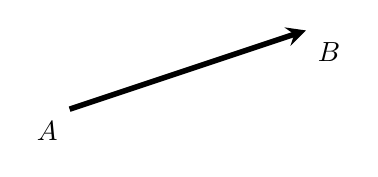
\begin{tikzpicture}
\draw[line width=2pt,-stealth](-1,0)node[below left]{$A$}--(2,1)node[below right]{$B$};
 \end{tikzpicture}
\end{image}
We refer to this vector as $\overrightarrow{AB}$.

\section*{Vectors in Standard Position}
Vectors that point in the same direction and have the same length are said to be \dfn{equivalent}.  For example, vectors  $\vec{u}$, $\vec{v}$ and $\vec{w}$ in the figure below are equivalent.  We write $\vec{u}=\vec{v}=\vec{w}$.

 \begin{image}[2.5in]
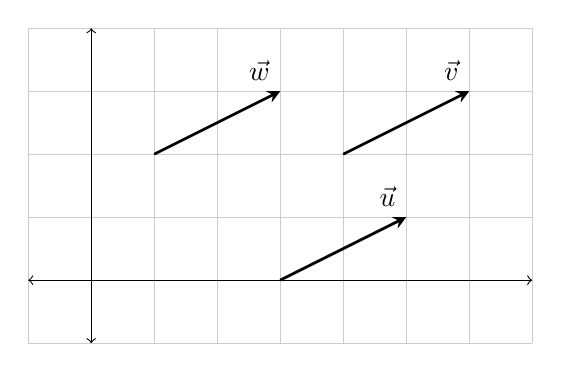
\begin{tikzpicture}[scale=0.8]
\draw[thin,gray!40] (-1,-1) grid (7,4);
  \draw[<->] (-1,0)--(7,0);
  \draw[<->] (0,-1)--(0,4);
  
 \draw[line width=1pt,-stealth](3,0)--(5,1)node[above left]{$\vec{u}$};
 \draw[line width=1pt,-stealth](4,2)--(6,3)node[above left]{$\vec{v}$};
 \draw[line width=1pt,-stealth](1,2)--(3,3)node[above left]{$\vec{w}$};
  %\draw[line width=2pt,red,-stealth](0,0)--(2,1) node[above right]{$[2,1]$};
 \end{tikzpicture}
\end{image}
 
For the purpose of developing standard, convenient notation, we observe that every vector is equivalent to some vector whose tail is at the origin.  Vectors with tails at the origin are said to be in \dfn{ standard position}.  We will refer to each vector in standard position by the coordinates of its head.   For example, a vector in standard position whose head is located at the point $(2, 1)$ will be referred to as $[2, 1]$.  

\begin{image}[2.5in]
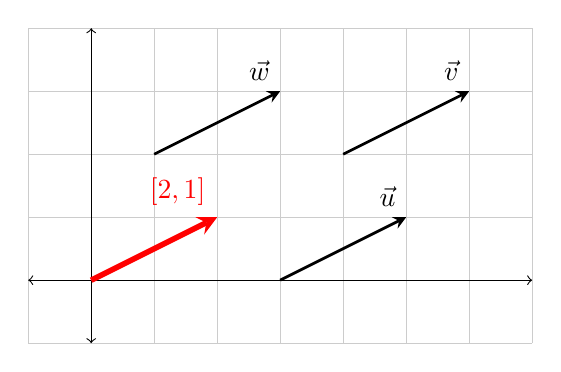
\begin{tikzpicture}[scale=0.8]
\draw[thin,gray!40] (-1,-1) grid (7,4);
  \draw[<->] (-1,0)--(7,0);
  \draw[<->] (0,-1)--(0,4);
  
 \draw[line width=1pt,-stealth](3,0)--(5,1)node[above left]{$\vec{u}$};
 \draw[line width=1pt,-stealth](4,2)--(6,3)node[above left]{$\vec{v}$};
 \draw[line width=1pt,-stealth](1,2)--(3,3)node[above left]{$\vec{w}$};
  \draw[line width=2pt,red,-stealth](0,0)--(2,1) node[above left]{$[2,1]$};
 \end{tikzpicture}
\end{image}



Vectors $\vec{u}, \vec{v}$ and $\vec{w}$ in the figure are equivalent to vector $[2,1]$.  We write $\vec{u}=\vec{v}=\vec{w}=[2,1]$.  Number $2$ is called the \dfn{first component} of the vector (or the $x$-component) while number $1$ is the \dfn{second component} (or the $y$-component).  The form $[2, 1]$ is called the \dfn{component form}.  

Vector $[2, 1]$ is an example of a \dfn{row vector}.  Later we will find that representing this vector as a \dfn{column vector} $\begin{bmatrix}
2\\
1
 \end{bmatrix}$ is often more convenient.

Column (or row) representation of vectors in component form allows us to go beyond the physical and geometric definition, and think of vectors more abstractly as arrays of numbers.

Our next goal is to find a process for writing any vector in the coordinate plane in component form.  
\begin{initprob}\label{init:headminustail}
Consider vector $\vec{v}$ shown below.  We will express $\vec{v}$ in component form.

\begin{image}[2in]
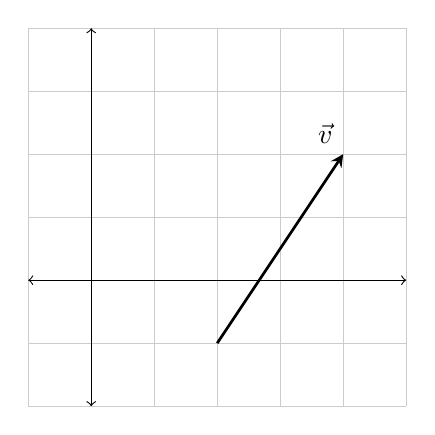
\begin{tikzpicture}[scale=0.8]
\draw[thin,gray!40] (-1,-2) grid (5,4);
  \draw[<->] (-1,0)--(5,0);
  \draw[<->] (0,-2)--(0,4);
  
 \draw[line width=1pt,-stealth](2, -1)--(4, 2)node[above left]{$\vec{v}$};
 
%  \draw[line width=2pt,red,-stealth](0,0)--(2,3) node[above left]{$[2,3]$};
 \end{tikzpicture}
\end{image}

Note that the vector has a ``run" of $2$ and a ``rise" of $3$.  If we construct a vector with tail at the origin, a ``run" of $2$ and a ``rise" of $3$, we will have a vector in standard position equivalent to vector $\vec{v}$.
\begin{image}[2in]
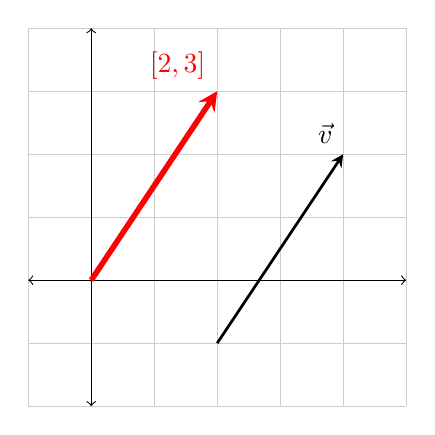
\begin{tikzpicture}[scale=0.8]
\draw[thin,gray!40] (-1,-2) grid (5,4);
  \draw[<->] (-1,0)--(5,0);
  \draw[<->] (0,-2)--(0,4);
  
 \draw[line width=1pt,-stealth](2, -1)--(4, 2)node[above left]{$\vec{v}$};
 
 \draw[line width=2pt,red,-stealth](0,0)--(2,3) node[above left]{$[2,3]$};
 \end{tikzpicture}
\end{image}
The component form for the vector we constructed is $[2,3]$.  This gives us $\vec{v}=[2,3]$.

The approach we used is applicable to specific vectors that can easily be visualized.  What we need is an algebraic approach that can be generalized to higher dimensions and more abstract situations.  

Suppose we were to slide vector $\vec{v}$ into standard position. Consider what would happen to the tail of $\vec{v}$ as we do so.
\begin{image}[2in]
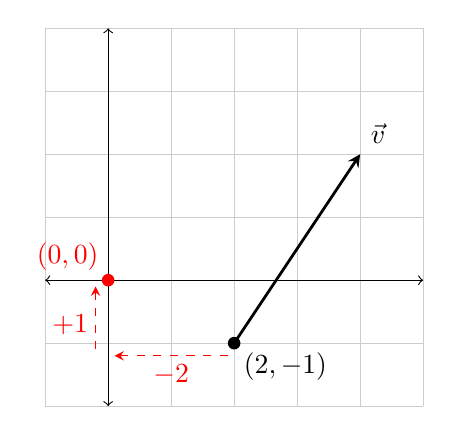
\begin{tikzpicture}[scale=0.8]
\draw[thin,gray!40] (-1,-2) grid (5,4);
  \draw[<->] (-1,0)--(5,0);
  \draw[<->] (0,-2)--(0,4);
  
 \draw[line width=1pt,-stealth](2, -1)--(4, 2)node[above right]{$\vec{v}$};
 \fill[black] (2,-1)node[below right]{$(2,-1)$} circle (0.1cm);
 
 \draw[line width=0.5pt,-stealth, dashed, red](1.9, -1.2)--(0.1,-1.2);
 \node[red] at (1, -1.5)   (a) {$-2$};
 
 
 \draw[line width=0.5pt,-stealth, dashed, red](-0.2, -1.1)--(-0.2, -0.1);
 \node[red] at (-0.6, -0.7)   (b) {$+1$};
 
 \fill[red] (0,0)node[above left]{$(0,0)$} circle (0.1cm);
 
% \draw[line width=2pt,red,-stealth](0,0)--(2,3) node[above left]{$[2,3]$};
 \end{tikzpicture}
\end{image}
What happens to the tail of the vector has to happen to the head

\begin{image}[2in]
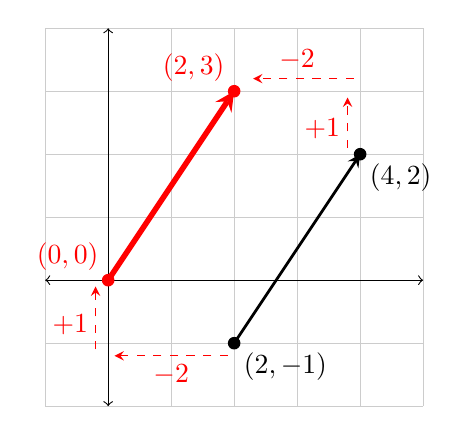
\begin{tikzpicture}[scale=0.8]
\draw[thin,gray!40] (-1,-2) grid (5,4);
  \draw[<->] (-1,0)--(5,0);
  \draw[<->] (0,-2)--(0,4);
  
 \draw[line width=1pt,-stealth](2, -1)--(4, 2);
 \fill[black] (2,-1)node[below right]{$(2,-1)$} circle (0.1cm);
 \fill[black] (4,2)node[below right]{$(4,2)$} circle (0.1cm);
 
 \draw[line width=0.5pt,-stealth, dashed, red](1.9, -1.2)--(0.1,-1.2);
 \node[red] at (1, -1.5)   (a) {$-2$};
 \draw[line width=0.5pt,-stealth, dashed, red](-0.2, -1.1)--(-0.2, -0.1);
 \node[red] at (-0.6, -0.7)   (b) {$+1$};
 
  \draw[line width=0.5pt,-stealth, dashed, red](3.9, 3.2)--(2.3,3.2);
 \node[red] at (3, 3.5)   (a) {$-2$};
 \draw[line width=0.5pt,-stealth, dashed, red](3.8, 2.1)--(3.8, 2.9);
 \node[red] at (3.4, 2.4)   (b) {$+1$};
 
 \fill[red] (0,0)node[above left]{$(0,0)$} circle (0.1cm);
 \fill[red] (2,3)node[above left]{$(2,3)$} circle (0.1cm);
 
 \draw[line width=2pt,red,-stealth](0,0)--(2,3);
 \end{tikzpicture}
\end{image}

We subtracted $2$ from the $x$-coordinate and added $1$ to the $y$-coordinate of the tail. To find the new location of the head we subtract $2$ from the $x$-coordinate of the head, and add $1$ to the $y$-coordinate of the head.  This gives us  $(4-2, 2+1)$.  So, the new location of the head is $(2, 3)$, and $\vec{v}=[2, 3]$.

If you look back at what we did you will find that the components of $\vec{v}$ were computed by subtracting the coordinates of the tail from the coordinates of the head
$$\vec{v}=[4-2, 2-(-1)]=[2, 3]$$
\end{initprob}

\begin{general}
The following diagram summarizes and generalizes our findings in Exploration Problem \ref{init:headminustail}.

Let $\overrightarrow{AB}$ be a vector in $\RR^2$, with tail at point $A(a_1, a_2)$ and head at point $B(b_1, b_2)$.

As we slide $\overrightarrow{AB}$ into standard position by moving point $A$ to the origin, point $B$ travels along with point $A$ by undergoing the same horizontal and vertical shifts. 

\begin{image}[2.5in]
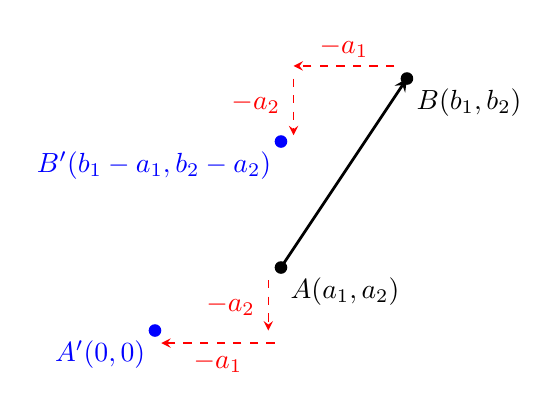
\begin{tikzpicture}[scale=0.8]
 % \draw[<->] (-1,0)--(5,0);
  %\draw[<->] (0,-1)--(0,5);
  
 \draw[line width=1pt,-stealth](2, 1)--(4, 4);
 \fill[black] (2,1)node[below right]{$A(a_1, a_2)$} circle (0.1cm);
 \fill[black] (4,4)node[below right]{$B(b_1, b_2)$} circle (0.1cm);
 
 \draw[line width=0.5pt,-stealth, dashed, red](1.9, -0.2)--(0.1,-0.2);
 \node[red] at (1, -0.5)   (a) {$-a_1$};
 \draw[line width=0.5pt,-stealth, dashed, red](1.8, 0.8)--(1.8, 0);
 \node[red] at (1.2, 0.4)   (b) {$-a_2$};
 
  \draw[line width=0.5pt,-stealth, dashed, red](3.8, 4.2)--(2.2,4.2);
 \node[red] at (3, 4.5)   (a) {$-a_1$};
 \draw[line width=0.5pt,-stealth, dashed, red](2.2, 4)--(2.2, 3.1);
 \node[red] at (1.6, 3.6)   (b) {$-a_2$};
 
 \fill[blue] (0,0)node[below left]{$A'(0,0)$} circle (0.1cm);
 \fill[blue] (2,3)node[below left]{$B'(b_1-a_1, b_2-a_2)$} circle (0.1cm);
 
 %\draw[line width=2pt,red,-stealth](0,0)--(2,3);
 \end{tikzpicture}
\end{image}
We now have an equivalent vector $\overrightarrow{A'B'}$ in standard position.
$$\overrightarrow{A'B'}=\overrightarrow{AB}=[b_1-a_1, b_2-a_2]$$ 
\end{general}

\begin{formula}
  [``Head - Tail'' Formula in $\RR^2$]\label{form:headminustailr2}
Suppose a vector's tail is at point $A(a_1, a_2)$ and the vector's head is at $B(b_1, b_2)$, then 
\begin{equation}\label{headtailr2}
\overrightarrow{AB}=[b_1-a_1, b_2-a_2]
\end{equation}
\end{formula}





\section*{Vectors in $\RR^3$}
Definitions of standard position and component form for vectors in $\RR^3$ are analogous to their counterparts for vectors in $\RR^2$.  For example, vector $\overrightarrow{OP}$ in the figure below, is in standard position and can be written in component form as $\overrightarrow{OP}=[6,10,7]$.

 \begin{image}[4in]
\begin{tikzpicture}[x=0.5cm,y=0.5cm,z=0.3cm]
% The axes
\draw[->] (xyz cs:x=-13.5) -- (xyz cs:x=13.5) node[above] {$y$};
\draw[->] (xyz cs:y=-13.5) -- (xyz cs:y=13.5) node[right] {$z$};
\draw[->] (xyz cs:z=13.5)--(xyz cs:z=-13.5) node[below] {$x$} ;
% The thin ticks
\foreach \coo in {-13,-12,...,13}
{
  \draw (\coo,-1.5pt) -- (\coo,1.5pt);
  \draw (-1.5pt,\coo) -- (1.5pt,\coo);
  \draw (xyz cs:y=-0.15pt,z=\coo) -- (xyz cs:y=0.15pt,z=\coo);
}

% Dashed lines for the points P
\draw[dashed,red] 
  (xyz cs:z=-6) -- 
  +(0,7) coordinate (u) -- 
  (xyz cs:y=7) -- 
  +(10,0) -- 
  ++(xyz cs:x=10,z=-6) coordinate (v) --
  +(0,-7) coordinate (w) --
  cycle;
\draw[dashed,red] (u) -- (v);
\draw[dashed,red] (10,7) -- (10,0) -- (w);

% Dots and labels for P
\node[fill,circle,inner sep=1.5pt,label={right:$P(6,10,7)$}] at (v) {};
\node[fill,circle,inner sep=1.5pt,label={above left:$O$}] at (0,0,0) {};

\draw[line width=2pt,-stealth, red](0,0,0)--(v);
\end{tikzpicture}
\end{image}

If a vector is not in standard position but the location of its head and tail are known, a three-dimensional version of the ``Head - Tail" formula can be used to express the vector in component form.


\begin{formula}
  [``Head - Tail'' Formula in $\RR^3$]\label{form:headminustailr3}
Suppose a vector's tail is at point $A(a_1, a_2, a_3)$ and the vector's head is at $B(b_1, b_2, b_3)$, then 
\begin{equation}\label{headtailr3}
\overrightarrow{AB}=[b_1-a_1, b_2-a_2,b_3-a_3]
\end{equation}
\end{formula}

\section*{Vectors in $\RR^n$}
We cannot see $\RR^n$ for $n>3$, but we can conceptualize it by generalizing what we know about $\RR^2$ and $\RR^3$.  A vector $\vec{v}$ in standard position whose head is located at $(v_1, v_2, \ldots ,v_n)$ can be written in component form as $\vec{v}=[v_1, v_2, \ldots ,v_n]$.  If the location of the head and the tail of the vector are given, then we can find the component form by using the generalized ``Head -  Tail" formula.

\begin{formula}
  [``Head - Tail'' Formula in $\RR^n$]\label{form:headminustailrn}
Suppose a vector's tail is at point $A(a_1, a_2, \ldots ,a_n)$ and the vector's head is at $B(b_1, b_2, \ldots ,b_n)$, then 
\begin{equation}\label{form:headtailrn}
\overrightarrow{AB}=[b_1-a_1, b_2-a_2, \ldots ,b_n-a_n]
\end{equation}
\end{formula}





\section*{Practice Problems}

\begin{problem}
Sketch each pair of vectors described below.  Express each vector in component form. 
  \begin{problem}
Vector $\vec{v}$ has a tail at $(-2,4)$ and a head at $(4,5)$. Vector $\vec{w}$ has a tail at $(8,-5)$ and a head at $(6,7)$.

Answer:
$$\vec{v}=[\answer{6}, \answer{1}]$$
$$\vec{w}=[\answer{-2}, \answer{12}]$$
\end{problem}

\begin{problem}
 Vector $\vec{v}$ has a tail at $(2,4,5)$ and a head at $(-2,4,8)$. Vector $\vec{w}$ has a tail at $(-3,4,5)$ and a head at $(7,7,8)$.
 
 Answer:
 $$\vec{v}=[\answer{-4},\answer{0},\answer{3}]$$
 $$\vec{w}=[\answer{10},\answer{3},\answer{3}]$$
 \end{problem}
  \end{problem}

\begin{problem}
Express vector $\vec{v}$ shown in the figure  in component form if the magnitude (length) of $\vec{v}$ is $5$.

\begin{image}[2in]
\begin{tikzpicture}[scale=0.8]
%\draw[thin,gray!40] (-1,-1) grid (4,4);
  \draw[<->] (-1,0)--(5,0);
  \draw[<->] (0,-1)--(0,4);
  
 \draw[line width=1pt,-stealth](0, 0)--(4,3)node[above left]{$\vec{v}$};
 
 \draw[line width=0.5pt, dashed](4, 0)node[below]{$4$}--(4,3);
 
%  \draw[line width=2pt,red,-stealth](0,0)--(2,3) node[above left]{$[2,3]$};
 \end{tikzpicture}
\end{image}

Answer:
$$\vec{v}=[\answer{4},\answer{3}]$$
\end{problem}

\begin{problem} Let $A(-2, 3)$, $B(3, 1)$ and $C(-1, -1)$.  Find point $D$ such that $\overrightarrow{AB}=\overrightarrow{CD}$.

Answer:
$$D(\answer{4}, \answer{-3})$$
\end{problem}

\end{document} 